\subsection{Methodologies and Experiments}
Cerezo et al. have pointed out that Barren Plateaus are cost function dependent \cite{cerezoCostFunctionDependent2021}, implying that the only way to eliminate Barren Plateaus is to use a local cost function with a shallow circuit.
However, other approaches can still mitigate the phenomenon without using the local cost function.
Skolik et al. and Liu et al. \cite{skolikLayerwiseLearningQuantum2021, liuParameterInitializationMethod2021} suggest that we can initiate the starting parameters away from plateaus to guarantee the trainability from the first steps.
In this section, we design the methodologies for the experiment to answer the research question.

\subsubsection{Research Context}
The VQA approach is the answer to many constraints of the NISQ device. It allows the construction of trainable circuits that receive the trainable parameters $\theta$.
VQA is known for many applications in optimisation and machine learning.
However, we have observed the existence of Barren Plateaus, causing the variance of the cost function gradient to vanish exponentially with the number of qubits.
In the literature review, we have investigated three methods \cite{cerezoCostFunctionDependent2021, liuParameterInitializationMethod2021, skolikLayerwiseLearningQuantum2021} to mitigate this phenomenon.
We answer the research question by conducting technology-oriented empirical research.
We summarise designed the process as Figure \ref{Research Activities}:

\begin{figure}
    \centering
    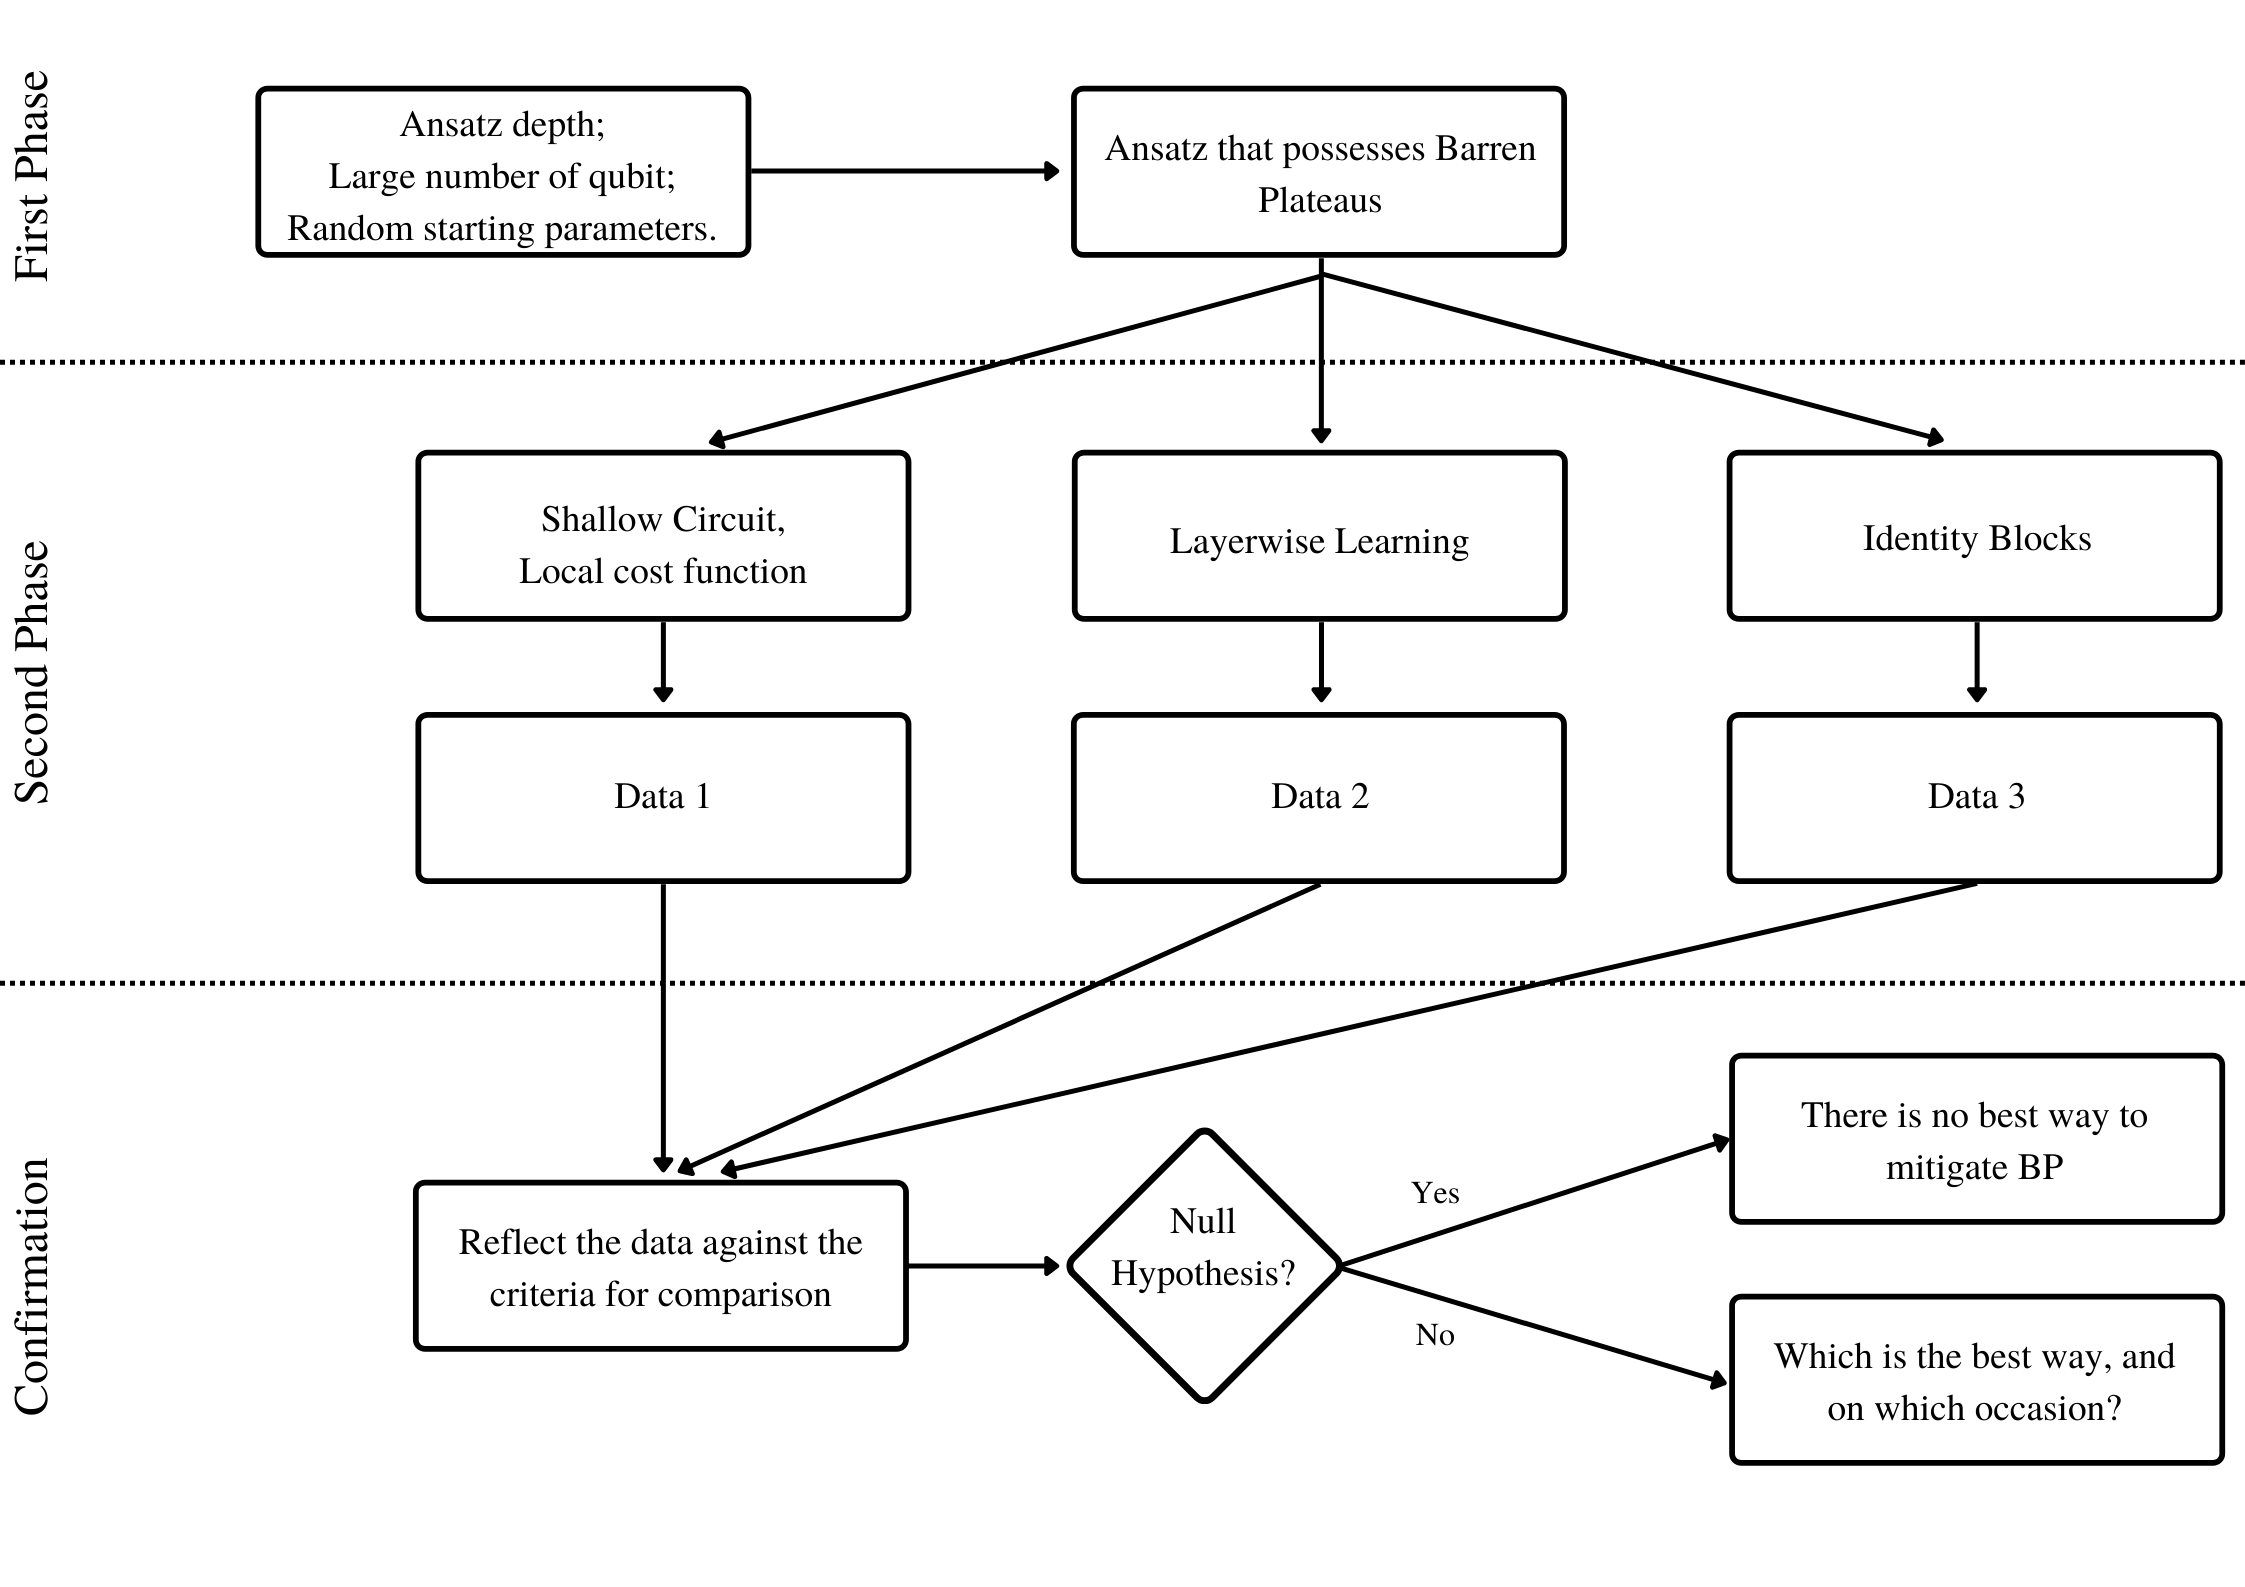
\includegraphics[width=\textwidth]{./ResearchDesign/Appendices/Method.png}
    \caption{
        Research method in summary.
    }
    \label{Research Activities}
\end{figure}

\subsubsection{Objects and Parameters}

As per the context, we can identify the object of study of this research to compare different BP mitigation methods against different ansatz designs.
One advantage of the empirical experiment is that we can have total control of the experiment environment.
In the context of this research, the parameters that we can vary are:
\begin{itemize}
    \item \textbf{The ansatz designs.} We have chosen the ansatzes NLocal and TwoLocal from Qiskit.
    \item \textbf{The ansatz configuration.} The ansatz object from Qiskit is mutable, which means we can configure their properties to fit the experiment activities. For example, the number of qubits, repetition of layers, and initial parameters.
    \item \textbf{The method to mitigate BP.} We have reviewed three methods in the literature review, and each of them has configured or trained the ansatz differently.
\end{itemize}

\subsubsection{Research Activities}
\textbf{In the first phase, we reproduce the Barren Plateaus.}
We can use Qiskit \cite{Qiskit} to construct an ansatz in a quantum simulator.
The literature review had pointed out that the two factors causing Barren Plateaus are the \textit{ansatz depth, a large number of qubits} and the \textit{randomised starting parameters}, so we configure the ansatzes to have such characteristics in a quantum simulator.
The optimisation algorithm will be the same in the ansatzes because the main concern is the three methods implemented in the second phase.
We keep track of the variance and the number of qubits to see if the variance is shrinking  \textit{exponentially} (see Figure \ref{Variance Shrinking demo}).
The result of the first phase is the ansatzes that possess Barren Plateaus.

\textbf{In the second phase, we implement the three approaches}.
With the QNN ansatzes from the first step, we can implement the three methods discussed in the literature review.
Each of them configures or trains the ansatz differently.
The Qiskit framework also supports the mutation for the ansatz object, such as the number of qubits to measure, the depth of ansatz (repetition) and the starting parameters.
We will track the variances of the gradient for each method to identify if the model has mitigated the Barren Plateaus phenomenon.
The output is recorded to compare against some criteria (the size of the circuit, execution time, etc.). We expect to have six outcomes.

The results of the research activities are discussed in the Subsection \ref{Data Collecting Section}.

\label{Research Activities section}
\begin{figure}
    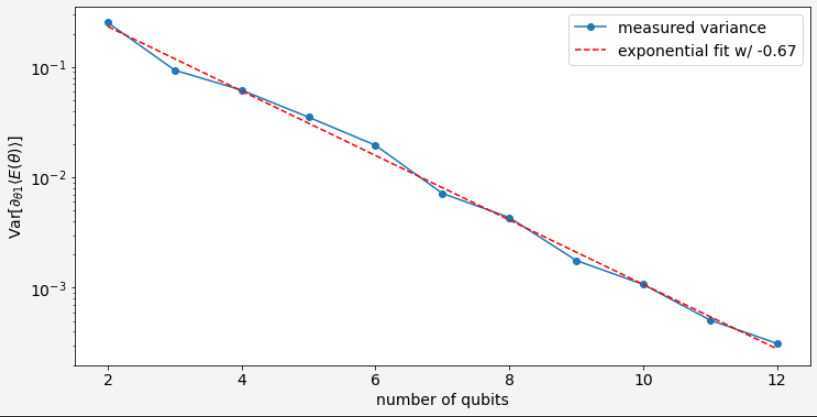
\includegraphics[width=\textwidth]{./ResearchDesign/Appendices/VarianceShrinking.png}
    \caption{
        An example of the Barren Plateaus phenomenon occurs in a QNN model.
        The variance of the gradient shrinks \textit{exponentially} with the number of qubits.
        Barren Plateaus phenomenon prevents optimisation algorithms from navigating the cost function landscape efficiently.
    }
    \label{Variance Shrinking demo}
\end{figure}


\subsubsection{Criteria}
\label{Criteria section}
We can compare the data with these criteria:
\begin{itemize}
    \item The quality of the solution;
    \item The size of the circuit;
    \item The size of the qubit registry;
    \item The time required to execute the circuit.
\end{itemize}

\subsubsection{Hypothesis}
The experiment activities are formalised into hypotheses:
\begin{itemize}
    \item \textbf{Null}: The three methods have the same performance according to the criteria, or the difference is insignificant;
    \item \textbf{Alternative}: The three methods' performance differs when reflecting the result against the criteria. If so,
          \begin{itemize}
              \item \textbf{H1}: We can identify which method is the best in specific criteria;
              \item \textbf{H2}: We can recommend the best approach given a context.
          \end{itemize}
\end{itemize}

\subsubsection{Data Collecting Method}
\label{Data Collecting Section}
Here we discuss our method to collect the data from the experiment.

The output of the first phase is Qiskit ansatz objects that contain the number of qubits, the depth of the circuit (rep), and the parameter configured randomly. Please refer to the Qiskit document for further detail.
Moreover, the ansatz object in Qiskit is mutable, which means we can modify the ansatzes properties in the second phase.

For the second phase, we need to record three different outputs of the three methods accordingly, with the criteria defined in Subsection \ref{Criteria section}.
The result is a table with the rows of criteria in the Subsection \ref{Criteria section} with each method as rows.
With this data, we can decide whether to reject the null hypothesis or not.

For the null hypothesis case, it means that the methods' performances are relatively the same, and we conclude the experiment.
We will have the result as a table for comparison, which satisfies hypothesis H1.
Then, we need to synthesise the table to answer the research question and verify hypothesis H2.
For example, the method $X$ is the best for the complexity.

Finally, we summarise the research results and present the findings.

\subsubsection{Resources}
Most of our required resources are open-sources:
\begin{itemize}
    \item Python 3.6+: \url{https://www.python.org/downloads/}
    \item Jupyter Notebook: \url{https://jupyter.org/}
    \item Qiskit: \url{https://qiskit.org/}
    \item IBM Quantum: \url{https://quantum-computing.ibm.com/}
    \item Qiskit circuit library: \url{https://qiskit.org/documentation/apidoc/circuit_library.html}
\end{itemize}

To prepare the quantum emulator on a local machine, we first install Python and Anaconda for programming language support and Jupyter Notebook as a code editing tool.
Then we follow the official instruction from Qiskit \cite{Qiskit} to install the necessary packages.
We can start working with Qiskit in a Jupyter Notebook file.

The other option is to use the provided Python kernel with Qiskit pre-installed provided by IBM Quantum.
While this is a convenient choice for online presentation or remote working because of instant access, this server has shortcomings.
The maximum ram for open access is only 8 Gigabytes, and the processing power is limited.

The quantum emulator from Qiskit is capable of simulating up to 32 qubits.
On the other hand, the actual quantum hardware from IBM is limited to 5 qubits for open access.

Qiskit has offered various ansatz designs, namely \textit{EfficientSU2, PauliTwoDesign, RealAmpplitudes, NLocal}, and \textit{TwoLocal}.
They are popular and frequently studied in quantum chemistry, quantum machine learning, and especially the investigation of Barren Plateaus.
However, they are based on the two ansatzes, NLocal and TwoLocal.
To construct the ansatz as discussed in Section \ref{Research Activities section}, we can use the NLocal and TwoLocal circuits provided.


\subsubsection{Success Condition}
The experiment will be concluded when these conditions are met:
\begin{itemize}
    \item We have QNN ansatzes that can produce Barren Plateaus;
    \item The three methods are implemented as Python scripts and ready for demonstration;
    \item The data from the three methods are evaluated against the criteria;
    \item We have identified when to use which method to counter Barren Plateaus.
\end{itemize}